% \documentclass{beamer}
% \usepackage{graphicx}
% \usepackage{multicol}
% \setlength{\columnseprule}{1pt}
%
% \graphicspath{{./fig/}}
% \usetheme{material}
% %%%%%%%%%%%%%%%%%%%%%%%%%%%%%%%%%%%%%%%%%%%%%%%%%%%%%%%%%%%%%%%%%%%%%%%%%%%%%%
% \embedvideo{<poster or text>}{<video file (MP4+H264)>}
% \embedvideo*{...}{...}                     % auto-play
%%%%%%%%%%%%%%%%%%%%%%%%%%%%%%%%%%%%%%%%%%%%%%%%%%%%%%%%%%%%%%%%%%%%%%%%%%%%%%

\ExplSyntaxOn
\NewDocumentCommand\embedvideo{smm}{
  \group_begin:
  \leavevmode
  \tl_if_exist:cTF{file_\file_mdfive_hash:n{#3}}{
    \tl_set_eq:Nc\video{file_\file_mdfive_hash:n{#3}}
  }{
    \IfFileExists{#3}{}{\GenericError{}{File~`#3'~not~found}{}{}}
    \pbs_pdfobj:nnn{}{fstream}{{}{#3}}
    \pbs_pdfobj:nnn{}{dict}{
      /Type/Filespec/F~(#3)/UF~(#3)
      /EF~<</F~\pbs_pdflastobj:>>
    }
    \tl_set:Nx\video{\pbs_pdflastobj:}
    \tl_gset_eq:cN{file_\file_mdfive_hash:n{#3}}\video
  }
  %
  \pbs_pdfobj:nnn{}{dict}{
    /Type/RichMediaInstance/Subtype/Video
    /Asset~\video
    /Params~<</FlashVars (
      source=#3&
      skin=SkinOverAllNoFullNoCaption.swf&
      skinAutoHide=true&
      skinBackgroundColor=0x5F5F5F&
      skinBackgroundAlpha=0
    )>>
  }
  %
  \pbs_pdfobj:nnn{}{dict}{
    /Type/RichMediaConfiguration/Subtype/Video
    /Instances~[\pbs_pdflastobj:]
  }
  %
  \pbs_pdfobj:nnn{}{dict}{
    /Type/RichMediaContent
    /Assets~<<
      /Names~[(#3)~\video]
    >>
    /Configurations~[\pbs_pdflastobj:]
  }
  \tl_set:Nx\rmcontent{\pbs_pdflastobj:}
  %
  \pbs_pdfobj:nnn{}{dict}{
    /Activation~<<
      /Condition/\IfBooleanTF{#1}{PV}{XA}
      /Presentation~<</Style/Embedded>>
    >>
    /Deactivation~<</Condition/PI>>
  }
  %
  \hbox_set:Nn\l_tmpa_box{#2}
  \tl_set:Nx\l_box_wd_tl{\dim_use:N\box_wd:N\l_tmpa_box}
  \tl_set:Nx\l_box_ht_tl{\dim_use:N\box_ht:N\l_tmpa_box}
  \tl_set:Nx\l_box_dp_tl{\dim_use:N\box_dp:N\l_tmpa_box}
  \pbs_pdfxform:nnnnn{1}{1}{}{}{\l_tmpa_box}
  %
  \pbs_pdfannot:nnnn{\l_box_wd_tl}{\l_box_ht_tl}{\l_box_dp_tl}{
    /Subtype/RichMedia
    /BS~<</W~0/S/S>>
    /Contents~(embedded~video~file:#3)
    /NM~(rma:#3)
    /AP~<</N~\pbs_pdflastxform:>>
    /RichMediaSettings~\pbs_pdflastobj:
    /RichMediaContent~\rmcontent
  }
  \phantom{#2}
  \group_end:
}
\ExplSyntaxOff
%
%% \newlength{\wdth}
%
%% \newcommand{\strike}[1]{\settowidth{\wdth}{#1}\rlap{\rule[.5ex]{\wdth}{.4pt}}#1}
%
%
%\begin{document}

% %%%%%%%%%%%%%%%%%%%%%%%%%%%%%%%%%%%%%%%%%%%%%%%%%%%%%%%%%%%%%%%%%%%%%%%%%%%%%%
% \embedvideo{<poster or text>}{<video file (MP4+H264)>}
% \embedvideo*{...}{...}                     % auto-play
%%%%%%%%%%%%%%%%%%%%%%%%%%%%%%%%%%%%%%%%%%%%%%%%%%%%%%%%%%%%%%%%%%%%%%%%%%%%%%

\ExplSyntaxOn
\NewDocumentCommand\embedvideo{smm}{
  \group_begin:
  \leavevmode
  \tl_if_exist:cTF{file_\file_mdfive_hash:n{#3}}{
    \tl_set_eq:Nc\video{file_\file_mdfive_hash:n{#3}}
  }{
    \IfFileExists{#3}{}{\GenericError{}{File~`#3'~not~found}{}{}}
    \pbs_pdfobj:nnn{}{fstream}{{}{#3}}
    \pbs_pdfobj:nnn{}{dict}{
      /Type/Filespec/F~(#3)/UF~(#3)
      /EF~<</F~\pbs_pdflastobj:>>
    }
    \tl_set:Nx\video{\pbs_pdflastobj:}
    \tl_gset_eq:cN{file_\file_mdfive_hash:n{#3}}\video
  }
  %
  \pbs_pdfobj:nnn{}{dict}{
    /Type/RichMediaInstance/Subtype/Video
    /Asset~\video
    /Params~<</FlashVars (
      source=#3&
      skin=SkinOverAllNoFullNoCaption.swf&
      skinAutoHide=true&
      skinBackgroundColor=0x5F5F5F&
      skinBackgroundAlpha=0
    )>>
  }
  %
  \pbs_pdfobj:nnn{}{dict}{
    /Type/RichMediaConfiguration/Subtype/Video
    /Instances~[\pbs_pdflastobj:]
  }
  %
  \pbs_pdfobj:nnn{}{dict}{
    /Type/RichMediaContent
    /Assets~<<
      /Names~[(#3)~\video]
    >>
    /Configurations~[\pbs_pdflastobj:]
  }
  \tl_set:Nx\rmcontent{\pbs_pdflastobj:}
  %
  \pbs_pdfobj:nnn{}{dict}{
    /Activation~<<
      /Condition/\IfBooleanTF{#1}{PV}{XA}
      /Presentation~<</Style/Embedded>>
    >>
    /Deactivation~<</Condition/PI>>
  }
  %
  \hbox_set:Nn\l_tmpa_box{#2}
  \tl_set:Nx\l_box_wd_tl{\dim_use:N\box_wd:N\l_tmpa_box}
  \tl_set:Nx\l_box_ht_tl{\dim_use:N\box_ht:N\l_tmpa_box}
  \tl_set:Nx\l_box_dp_tl{\dim_use:N\box_dp:N\l_tmpa_box}
  \pbs_pdfxform:nnnnn{1}{1}{}{}{\l_tmpa_box}
  %
  \pbs_pdfannot:nnnn{\l_box_wd_tl}{\l_box_ht_tl}{\l_box_dp_tl}{
    /Subtype/RichMedia
    /BS~<</W~0/S/S>>
    /Contents~(embedded~video~file:#3)
    /NM~(rma:#3)
    /AP~<</N~\pbs_pdflastxform:>>
    /RichMediaSettings~\pbs_pdflastobj:
    /RichMediaContent~\rmcontent
  }
  \phantom{#2}
  \group_end:
}
\ExplSyntaxOff

\section{Applications}
\topicFramePrimary{Examples of applications that benefit from real-time 3D-PTV}

\begin{frame}[label=app-1]
\frametitle{Real-time flow information is beneficial in applications}
\begin{itemize}
	\item Time-varying on slow time scales
    \item Unpredictable start and duration 
    \item Irreproducible or expensive % add suction feeding stuff, ceramic particle release stuff, rupture and breakage
	\item Control of the flow-dependent process, or control the flow % add wind turbine stuff
    \item Mobile systems, field experiments
    \item Harsh environments, remote operation
\end{itemize}
\end{frame}

\begin{frame}[label=app-2]{Particle motion due to pressure change in loadlocks}
\centering\cardImg{lab1}{\textwidth}
\end{frame}

\begin{frame}[label=app-3]{We can leave the lab}
\begin{multicols}{2}
    \cardImg{ldc3}{.49\textwidth}
    \cardImg{ldc_splitter}{.49\textwidth}
\end{multicols}
\end{frame}


\begin{frame}[label=iibr-4]{3D flow inside canopy in a large scale Environmental Wind Tunnel}
\begin{columns}
\column{0.5\textwidth}
    \cardImg{wind_tunnel_photo_1}{1\textwidth}
%\end{frame}
%\begin{frame}[label=iibr-5]{We are ready for the Environmental Wind Tunnel}
\column{0.5\textwidth}
    \cardImg{ptv_wind_tunnel_photo1}{1\textwidth}
\end{columns}
\end{frame}

\begin{frame}[label=app-19]{Flow inside the canopy \href{https://www.dropbox.com/s/9x43i2uk9q38fho/flow_inside_laser.mp4?raw=1}{video}}
    \centering
    \embedvideo{\cardImg{flow_snapshot_inside.jpg}{.9\textwidth}}{video/flow_inside_laser.mp4}
\end{frame}
    

\begin{frame}[label=app-12]{The whole system can slide or rotate}
    \cardImg{sliding_ptv.jpg}{.9\textwidth}
    \begin{cardTiny} 
        Walpot et al. Meas. Sci. Tech. 2006. TU/e
    \end{cardTiny}
\end{frame}
    

\begin{frame}[label=app-6]{Rotation table experiments, \href{https://www.dropbox.com/s/933wsb9xdahbyi9/rotation.mp4?raw=1}{ETH Zurich}}
    \embedvideo{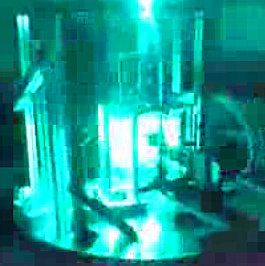
\includegraphics[width=0.8\textwidth]{fig/rotation.jpg}}{video/rotation.mp4}
\end{frame}
    
  
\begin{frame}[label=app-7]{Microgravity applications: remote and \href{https://www.dropbox.com/s/59ophf177gcfjzq/boiling_microgravity.mp4?raw=1}{difficult to control}}   
    % \begin{columns}
    % \column{.4\textwidth}
    %     \cardImg{microgravity}{\linewidth}
    % \column{.7\textwidth}
    \centering
    \embedvideo{\cardImg{space_3d_ptv}{.8\textwidth}}{video/boiling_microgravity.mp4}    
        
%    \end{columns}
\end{frame}


% \begin{frame}[label=app-11]{Real-time is easier with a single camera with a four-view splitter}
%     \centering\cardImg{ldc_splitter}{0.8\textwidth}
%     \embedvideo{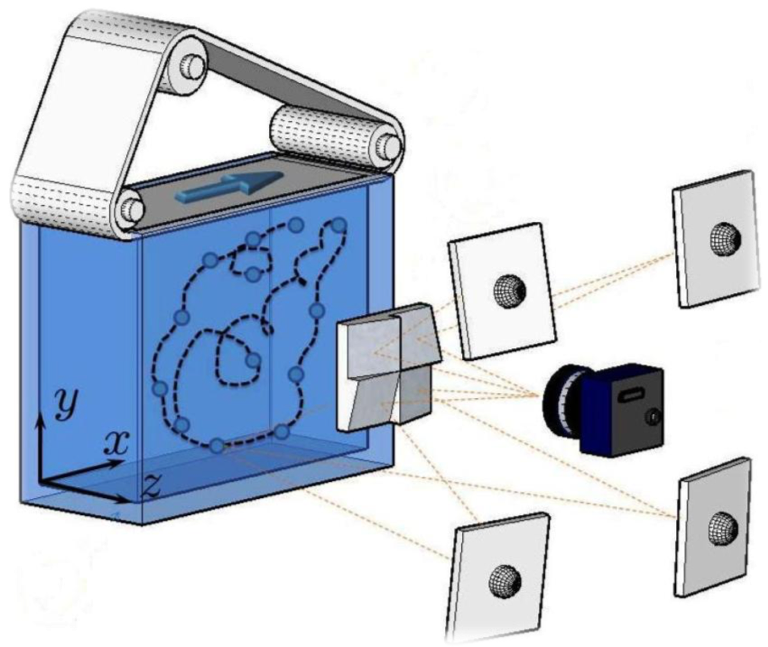
\includegraphics[width=\textwidth]{ldc_splitter}}{video/splitter_short.mp4}
%     % \begin{cardTiny} A high speed camera with a four-view optical system \end{cardTiny}
% \end{frame}

    
\begin{frame}[label=app-8]{An example from Chamorro's group}
    \centering\cardImg{kim/setup.png}{.9\textwidth}
\end{frame}
    
\begin{frame}[label=app-9]{Four view splitter \href{https://www.dropbox.com/s/h6g8d373lxgkqv8/Video1a.mp4?raw=1}{video}}
    \embedvideo{
\includegraphics[width=.8\textwidth]{fig/kim/4views.png}}{fig/kim/Video1a.mp4}
\end{frame}
    
% \begin{frame}[label=app-10]{You can get very dense result: turbulent jet}
%     \centering\cardImg{kim/jet.png}{\textwidth}
% \end{frame}

\begin{frame}[label=app-10b]{You can adjust 3D-PTV to microflows, using defocusing, scanning, photogrammetry}
\begin{center}
\begin{columns}
\column{.7\textwidth}
	\cardImg{kim/micro_3dptv.png}{\textwidth}
\column{.3\textwidth}
	\cardImg{kim/micro_3dptv_result.png}{\textwidth}
\end{columns}
\end{center}
\end{frame}


\begin{frame}[label=app-13]{Remote application and harsh environment: MRI + 3D-PTV}
    \begin{columns}
    \column{.5\textwidth}
        \cardImg{mri2}{.75\textwidth}
        \cardImg{mri3}{.75\textwidth}
    \column{.5\textwidth}
        \centering\cardImg{mri1}{\textwidth}
    \end{columns}
\end{frame}

\begin{frame}[label=app-14]{Biomedical applications: moving boundaries + complex geometries, \href{https://www.dropbox.com/s/p1xnc7mefoqboti/aorta_rigid.mp4?dl=0}{ETH Zurich}}
\embedvideo{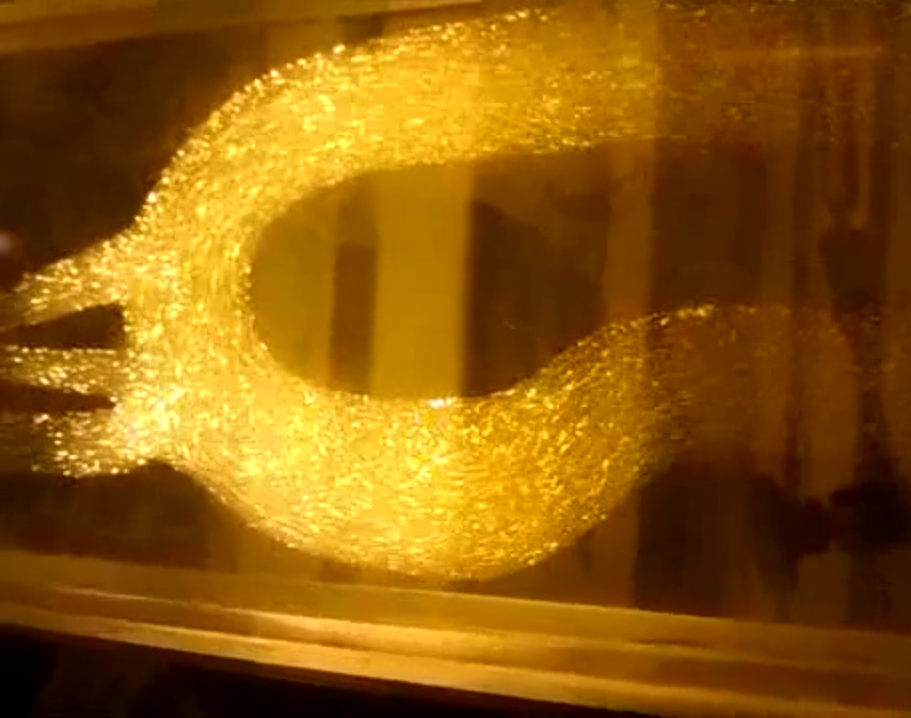
\includegraphics[width=\textwidth]{fig/aorta.png}}{video/aorta_rigid.mp4}
    \cardImg{aorta}{.9\textwidth}
\end{frame}

\begin{frame}[label=app-15]{Cerebrospinal fluid project -- \href{https://idsc.ethz.ch/research-guzzella-onder/research-projects/ProjectArchive/csf-biothermofluidics.html}{ETH Zurich}}
\embedvideo{\cardImg{brain}{\textwidth}}{video/brain.mp4}
\end{frame}
    
% \begin{frame}[label=iibr-16]{Camera system and laser}
%     \begin{multicols}{2}
%     \centering
%     \cardImg{camera_system_laser.jpg}{0.49\textwidth}
%     \cardImg{calibration_in_laser.jpg}{.49\textwidth}
%     \end{multicols}
%     \begin{cardTiny}
%     Four cameras point into the measurement location, as seen from the test section inside the tunnel, and the calibration target is mounted on the traverse arm.
%     \end{cardTiny}
% \end{frame}
    
%     %
% \begin{frame}[label=iibr-17]{Camera system and laser}
%     \begin{multicols}{2}
%     \centering\cardImg{img1.jpg}{.49\textwidth}
%     \cardImg{camera_system_laser.jpg}{0.49\textwidth}
%     \end{multicols}
% \end{frame}
    
    % \begin{frame}{Pressurized air seeding devices}
    % \cardImg{seeding_sources_2.jpg}{0.9\textwidth}
    % \end{frame}
    
    % \begin{frame}{Seeding material}
    % \centering\cardImg{SiO2_003}{0.75\textwidth}
    % \end{frame}
    
    
    % \subsection{3D Particle Tracking Velocimetry}
    
    %\begin{frame}
    %\centering\cardImg{volumes.png}{.6\textwidth}
    %\begin{cardTiny}
    %Representation in the isometric view of the measurement sub-volumes within and above the canopy layer. The arrow points in the streamwise direction.
    %\end{cardTiny}
    %\end{frame}
    
    
    % \begin{frame}[label=app-18]{Flow above the canopy}
    % \centering
    % \cardImg{flow_snapshot_above.jpg}{.9\textwidth}
    % \end{frame}
    
    % \begin{frame}[label=app-19]{Flow inside the canopy}
    % \centering
    % \cardImg{flow_snapshot_inside.jpg}{.9\textwidth}
    % \end{frame}
    
    % \begin{frame}[label=app-10]{\href{./fig/flow_inside_laser.mp4}{Video clip}}
    % \centering\cardImg{flow_snapshot_inside.jpg}{\textwidth}
    % \end{frame}
    
%    
%    

%    
%    
% \begin{frame}[label=app-21]{Take it to the space -- video credit: \href{https://www.dropbox.com/s/59ophf177gcfjzq/boiling_microgravity.mp4?raw=1}{ESA}}
%     %\cardImg{maser_8}{0.3\textwidth}
%     \embedvideo{\cardImg{space_3d_ptv}{0.8\textwidth}}{video/boiling_microgravity.mp4}
%     \begin{cardTiny}
%     Design and calibration of a four-headed camera for use in microgravity research, Willneff and Maas, ETH Zurich
%     \end{cardTiny}
% \end{frame}
    

\begin{frame}[label=app-22]
    \frametitle{Suction feeding events, courtesy of \href{https://www.dropbox.com/s/wcytdkxuxxvn4q0/fish_feeding.mp4?raw=1}{Prof. Roi Holzman, TAU}}
    \embedvideo{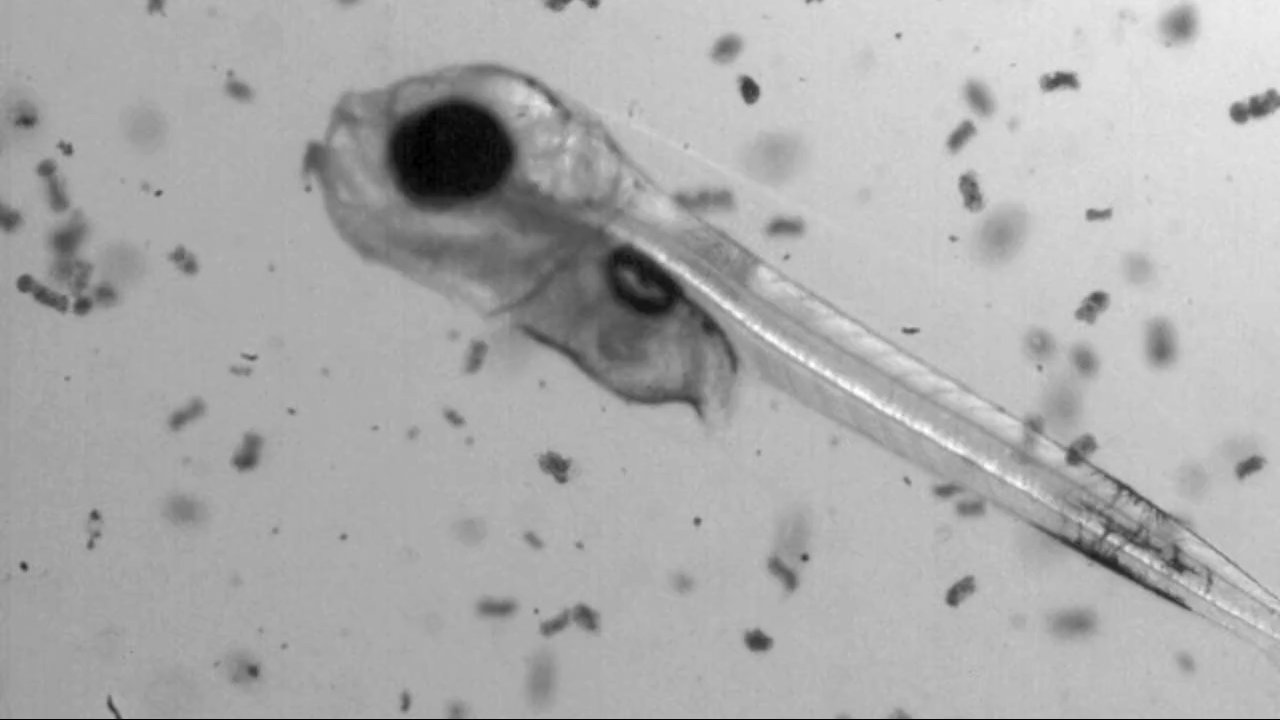
\includegraphics[width=\textwidth]{fig/fish_feeding.png}}{video/fish_feeding.mp4}
    %or this great video from Monterey Bay Aquarium 
    %
    %https://www.youtube.com/watch?v=umTqQSzKRmA    
\end{frame}
    
\begin{frame}[label=app-23]
    \frametitle{Flamingo underwater feeding -- \href{https://www.dropbox.com/s/ic0l5npzon834l9/flamingo.mp4?raw=1}{San Diego Zoo}}
    % https://www.youtube.com/watch?v=-1BF2XqboOo
    \begin{center}
    \embedvideo{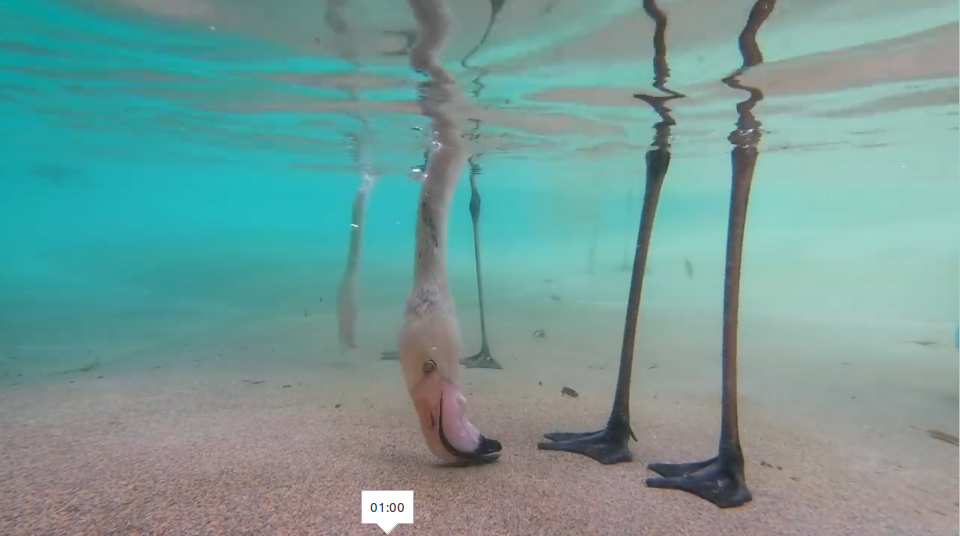
\includegraphics[width=\textwidth]{fig/flamingo.png}}{video/flamingo.mp4}
    \end{center}
\end{frame}
    
    %
    
\begin{frame}[label=app-24]
    \frametitle{Colloid aggregates breakage in extensional 3D flow, \href{https://www.dropbox.com/s/aufwfraotj5rll7/colloids1.mp4?raw=1}{ETH Zurich}}
    %https://pubs.acs.org/doi/10.1021/acs.langmuir.5b03804
\begin{center}
    \embedvideo{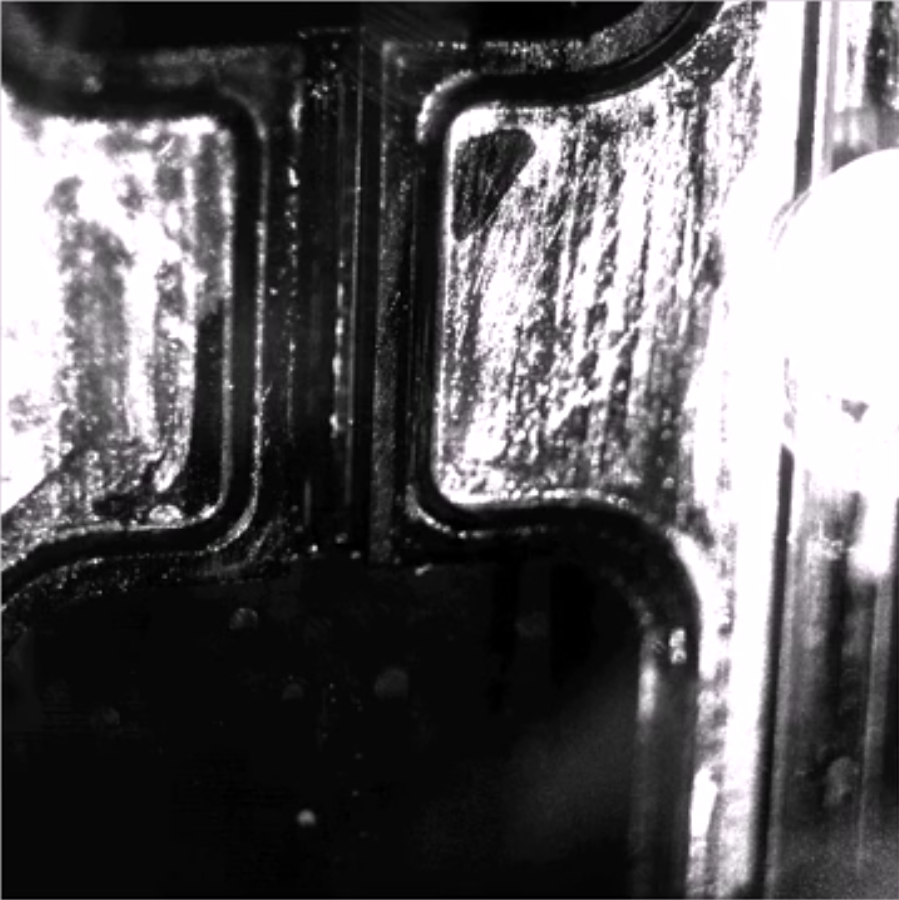
\includegraphics[width=\textwidth]{fig/colloids1.png}}{video/colloids1.mp4}
\end{center}    
\end{frame}
    
\begin{frame}[label=app-25]{Quantify colloid aggregates breakage in turbulence \href{https://www.dropbox.com/s/8cimpwfsukf11u2/colloids2.mp4?raw=1}{ETH Zurich}}
    %https://pubs.acs.org/doi/10.1021/acs.langmuir.5b03804
\begin{center}
    \embedvideo{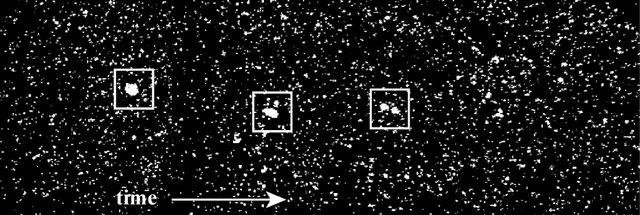
\includegraphics[width=\textwidth]{colloid_sequence.jpg}}{video/colloids2.mp4}
\end{center}       
\end{frame}
    
    
\begin{frame}[label=app-26]{Real-time vortex identification for wind turbine blade pitch control -- Caroline Braud}
    \begin{multicols*}{2}
    \cardImg{real_time_vortex_1}{.49\textwidth}
    \cardImg{real_time_vortex_2}{.49\textwidth}
    \end{multicols*}
\end{frame}
    
\begin{frame}[label=app-27]{Real-time sizing with 3D tracking -- Rayne Ramirez, Uni. Oslo}
  \begin{columns}
    \column{0.5\textwidth}
        \cardImg{drop-example}{\textwidth}
    \column{0.5\textwidth}
        \cardImg{drops}{\textwidth}
 \end{columns}
\end{frame}
    
\begin{frame}[label=app-28]{Fibers -- \href{https://www.dropbox.com/s/y5gf55qqeyq5ljr/fibers.mp4?raw=1}{Stefano Brizzolara, ETH Zurich}}
    % https://twitter.com/stebrizzo94/status/1525577322144976910?s=20
\begin{center}
    \embedvideo{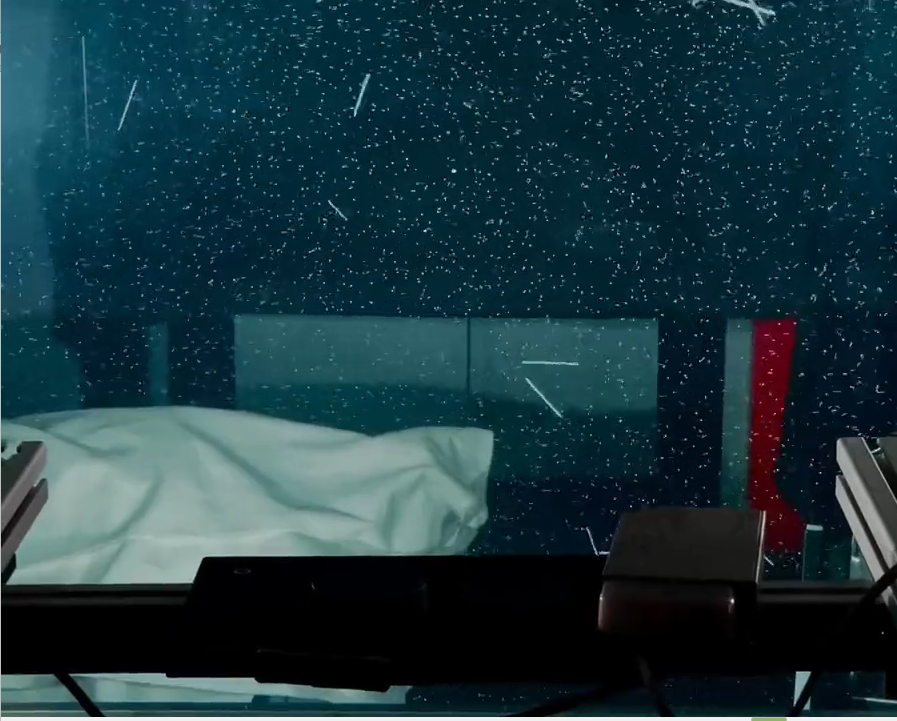
\includegraphics[height=0.8\textheight]{fibers.png}}{video/fibers.mp4}
\end{center}    
\end{frame}

\begin{frame}[label=app-29]{Microplastics in a vortex - \href{https://www.dropbox.com/s/in5ewv968dy9j3q/microplastics.mp4?raw=1}{Turbulence Structure Laboratory}}
    % Imaging‑based 3D particle tracking system forfield characterization ofparticle dynamics inatmospheric flows
    \embedvideo{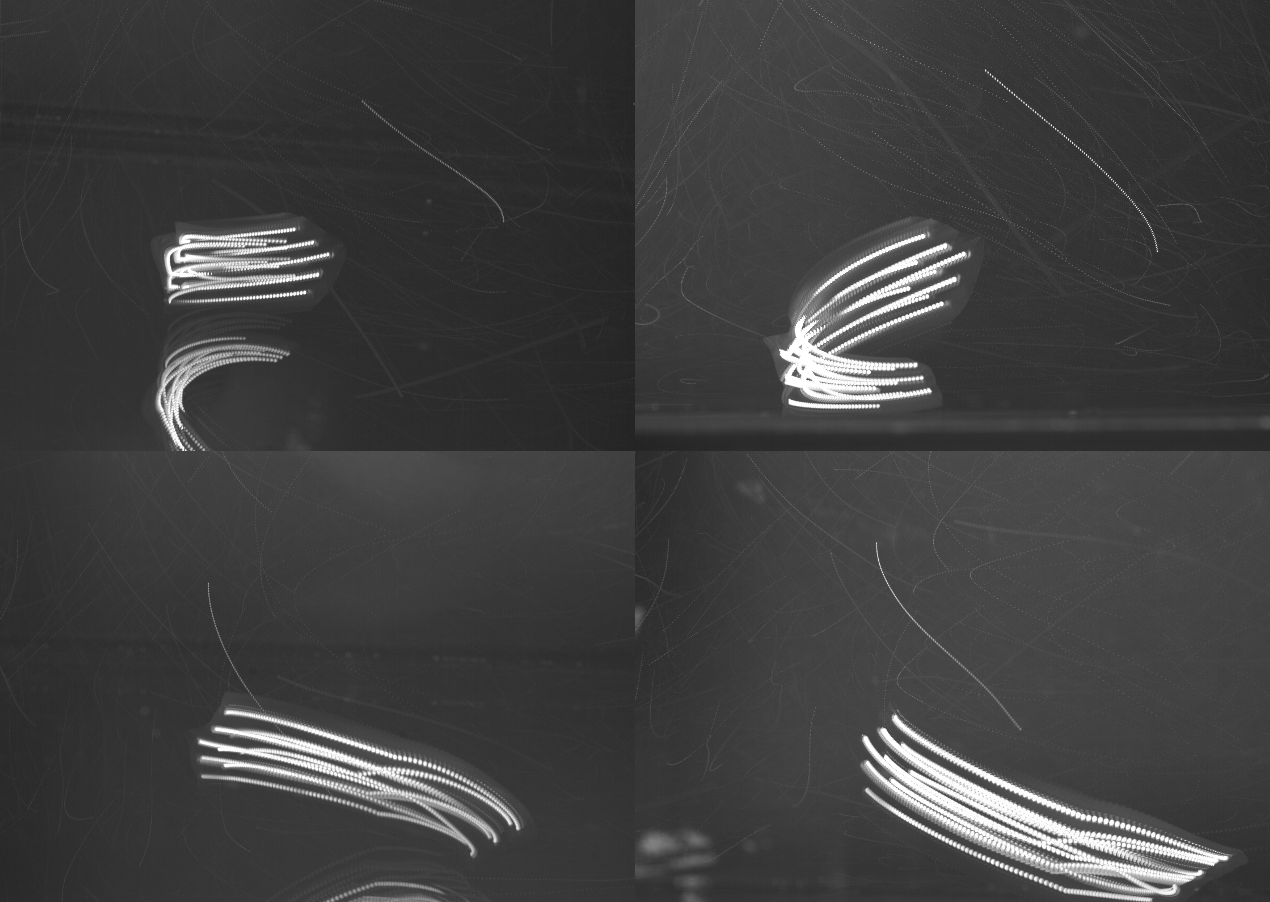
\includegraphics[height=\textheight]{trajects.png}}{video/microplastics2.mp4}\\
    Bristow et al. Exp. Fluids, 2023
\end{frame}

    
\begin{frame}[label=app-18a]{Multiphase flows - track both particles and flow, \href{}{inertial clustering}}
\begin{center}
    \embedvideo{\cardImg[height=.8\textheight]{two_phase_3dptv}
    {0.8\textwidth}}{video/twophase.mp4}
\end{center}
\end{frame}
    
    
\begin{frame}[label=app-30]{Drone vs turbulence - \href{https://www.dropbox.com/s/3lav5rf6s8su6f5/drone.mp4?raw=1}{University of Minnesota}}
    % Imaging‑based 3D particle tracking system forfield characterization ofparticle dynamics inatmospheric flows
    \begin{center}
    \embedvideo{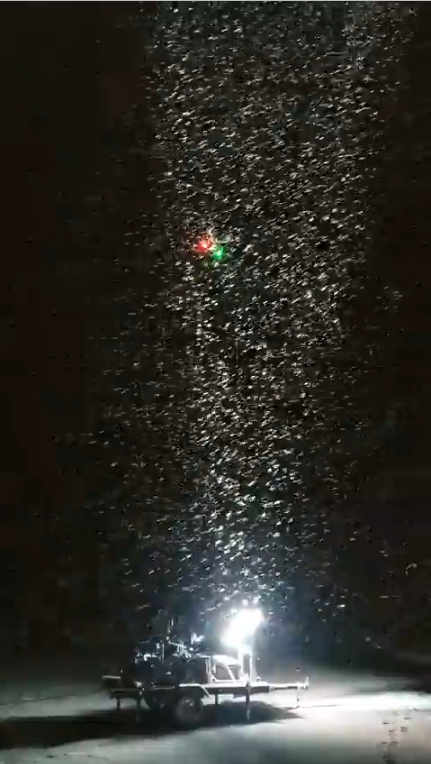
\includegraphics[height=0.8\textheight]{drone.png}}{video/drone.mp4}\\
    Bristow et al. Exp. Fluids, 2023
    \end{center}
\end{frame}
    
\begin{frame}[label=app-31a]{Soon we could do it using \href{https://www.dropbox.com/s/ckis9r6omd5y4fq/vuforia.mp4?raw=1}{AR/VR}}
    \centering 
    \embedvideo{\cardImg{mr_ptv_photo}{0.8\textwidth}}{video/vuforia.mp4}
    Chivers, T. Uni. Vermont, MSc Thesis, 2023 and Vuforia promotional video
\end{frame}

\begin{frame}[label=app-31b]{Real-time 3D-PTV is enabling technology for autonomous lab: \href{https://self-driving-lab-demo.readthedocs.io/en/latest/index.html}{self-driving-lab-demo.readthedocs.io}}
    \centering \cardImg[height=.75\textheight]{automatic_lab_concept}{\textwidth}
\end{frame}
        
    
% \begin{frame}[label=app-32]{Turbulent flow inside an urban canopy model at \href{https://www.dropbox.com/s/9x43i2uk9q38fho/flow_inside_laser.mp4?raw=1}{IIBR wind tunnel}}
%     \embedvideo{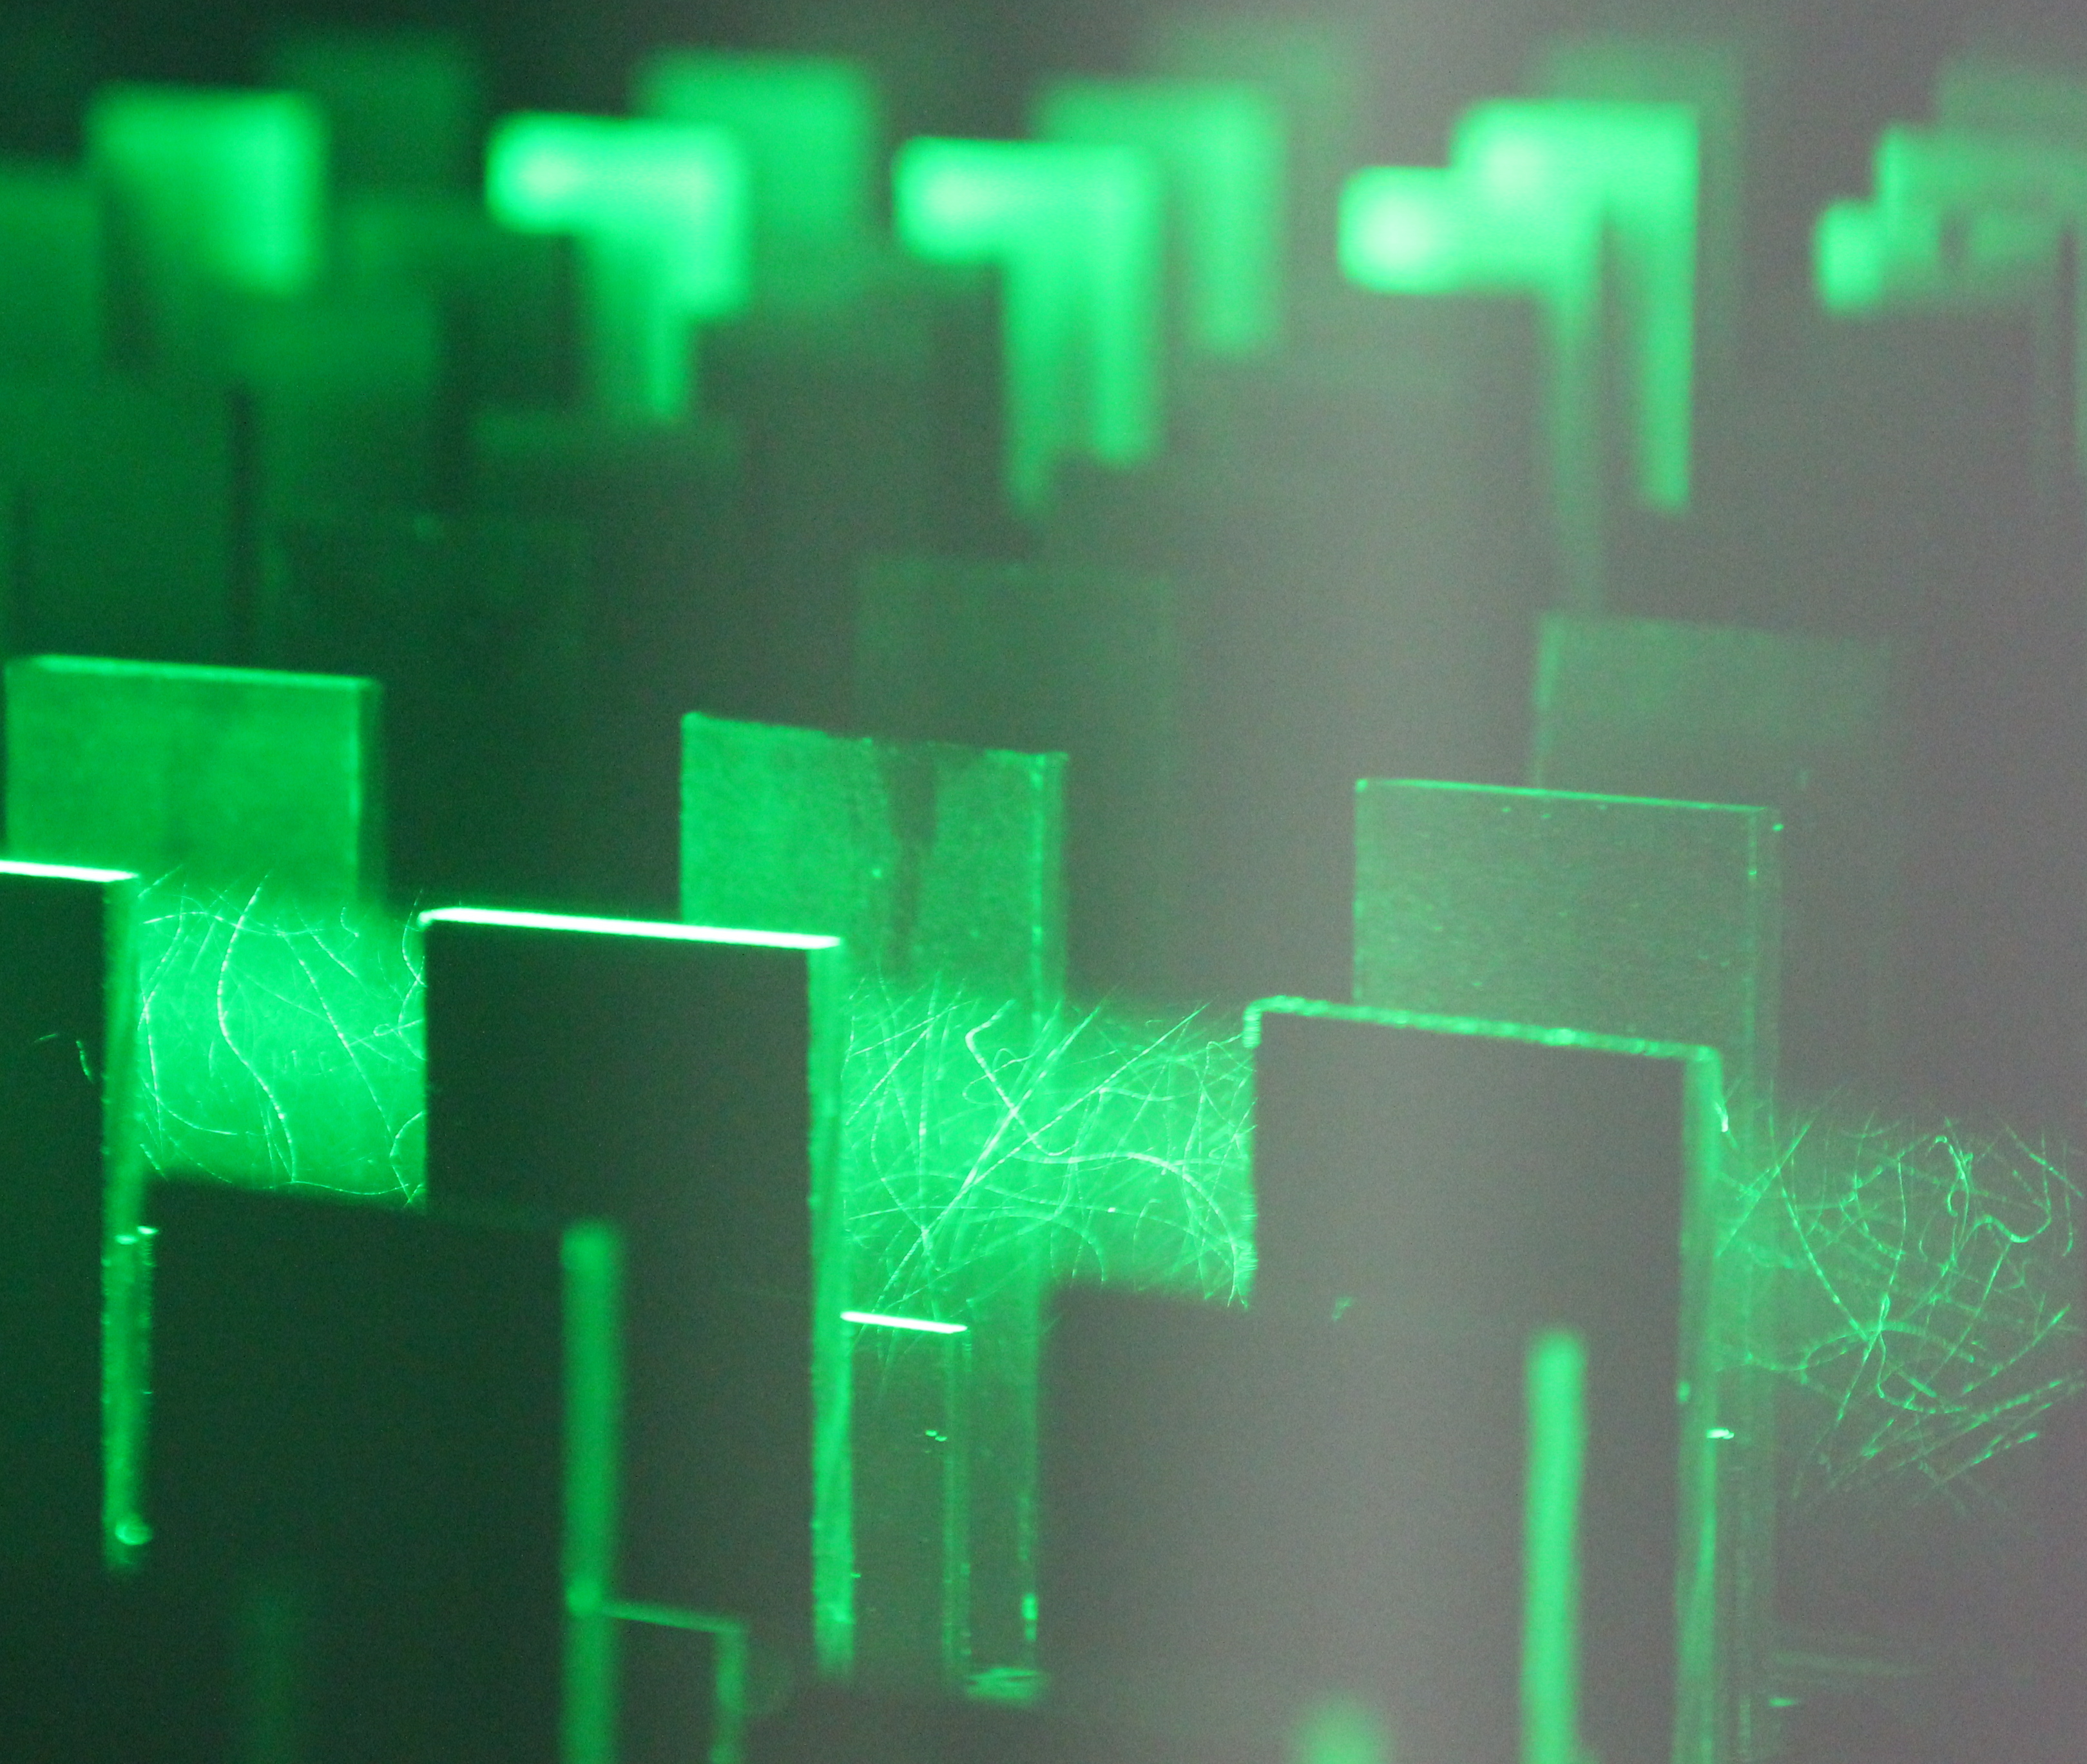
\includegraphics[width=\textwidth]{flow_snapshot_inside.jpg}}{video/flow_inside_laser.mp4}
% \end{frame}
%    

%\end{document}

\begin{frame}[label=app-20]{You could also do PIV on FPGA}
    \centering \cardImg[height=.75\textheight]{real_time_piv_fpga.png}{\textwidth}
    \begin{cardTiny}
    Real-time particle image velocimetry based on FPGA technology, Munoz et al. IEEE (2009)
    \end{cardTiny}
\end{frame}

    
\begin{frame}[label=app-17a]{But 3D-PTV can you give more insight in terms of 3D structure and turbulence}
    \begin{cardTiny} 
    This means we need  the \alert{full gradient tensor} along the particle trajectories:
    $\partial u_{i}/\partial x_{j}$ in space and time
    \end{cardTiny}
    \begin{multicols}{2}
    \centering
    \cardImg{moffatt2}{.49\textwidth}
    \cardImg{ptvgif}{.49\textwidth}
    \end{multicols}
\end{frame}
